\documentclass[tikz]{standalone}
\usetikzlibrary{automata, arrows.meta}

\begin{document}

\tikzset{
  node distance=2cm,
  state/.style={
    circle,
    thick,
    draw=black!75,
    minimum size=1cm
  },
  initial text=$\sigma$,
  accepting/.style={double},
  every edge/.style={
    ->,
    > =stealth',
    auto
  }
}

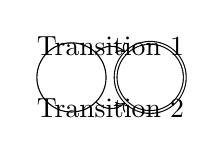
\begin{tikzpicture}[bend angle=45]

\node[state] (sigma) {};
\node[state, right of=sigma, accepting] (hat_sigma) {};

\path[->]
  (sigma) edge[bend left] node {Transition 1} (hat_sigma)
  (sigma) edge[bend right] node {Transition 2} (hat_sigma);

\end{tikzpicture}

\end{document}